% File project.tex
%% Style files for ACL 2021
\documentclass[11pt,a4paper]{article}
\usepackage[hyperref]{acl2021}
\usepackage{times}
\usepackage{booktabs}
\usepackage{todonotes}
\usepackage{latexsym}
\renewcommand{\UrlFont}{\ttfamily\small}
\usepackage{multirow}

% This is not strictly necessary, and may be commented out,
% but it will improve the layout of the manuscript,
% and will typically save some space.
\usepackage{microtype}

\aclfinalcopy 

\newcommand\BibTeX{B\textsc{ib}\TeX}

\title{11-777 Spring 2021 Class Project\\
Analysis of Baselines}

\author{
  Christian Deverall\thanks{\hspace{4pt}Everyone Contributed Equally -- Alphabetical order} \hspace{2em} Jingyuan Li $^*$ \hspace{2em} Artidoro Pagnoni $^*$ \\
  \texttt{\{cdeveral, jingyua4, apagnoni\}@andrew.cmu.edu}
  }

\date{}

\begin{document}
\maketitle

% sections: High level (explain seen vs unseen),  Segmentation, Action-level 

\section{Introduction}

As detailed in the Baselines and Metrics chapter, the baselines we evaluate are the ``Modular Object-Centric Approach'' (MOCA) \citep{singh2020moca} model and the ``Sequence-to-Sequence with Progress Monitor'' model (baseline of the ALFRED proposal paper) \citep{ALFRED20}. We often compare in two settings: ``seen'' and ``unseen''. ``Seen'' refers to when all the test tasks take place in rooms that have been previously seen in the training set. This chapter is split into a analysis of the action-sequences comparing baselines to the ground-truth sequences, an analysis of the predicted segmentation masks for interactive actions, an analysis of the errors leading to invalid actions, and an analysis of the performance of unimodal baselines. 

We use the published results from the two baselines to discuss the unimodal ablations (we did not retrain the unimodal models). However, we provide our results for the MOCA full model baseline confirming they are in line with the published results (Table \ref{tab:results}). We use this model to obtain the statistics discussed below. Setting up the environment (in particular AI2Thor) was not trivial, we used this assignment to successfully complete the setup.

Through our analysis we identify areas that could lead to performance improvements for the MOCA baseline.

% \begin{table*}[]
%     \centering
%     \begin{tabular}{c|c|c|c|c}
%     \toprule
%     & \multicolumn{2}{c|}{Seen} & \multicolumn{2}{c}{Unseen} \\
%     & Task (PW) & Goal-Cond (PW) & Task (PW) & Goal-Cond (PW) \\
%     \midrule
%     Seq2Seq + PM  & 3.7~(2.1) & 10.0~(10.0) & 0.0~(0.0) & 6.9~(5.1) \\ 
%     MOCA  & 19.2~(13.6) & 28.5~(22.3) & 3.8~(2.0) & 13.4~(8.3) \\
%     MOCA (ours) & 20.8~(14.4) & 29.7~(22.6) & 2.8~(1.4) & 12.8~(7.6) \\
%     \midrule
    
%     \bottomrule
%     \end{tabular}

% \end{table*}


% Please add the following required packages to your document preamble:
% \usepackage{multirow}
\begin{table*}[]
\begin{tabular}{ll|l|l|l|l|}
\cline{3-6}
                                              &                  & \multicolumn{2}{c|}{Seen}    & \multicolumn{2}{c|}{Unseen} \\ \cline{3-6} 
                                              &                  & Task (PW)   & Goal-Cond (PW) & Task (PW)  & Goal-Cond (PW) \\ \cline{2-6} 
\multicolumn{1}{l|}{}                         & Seq2Seq + PM     & 3.7 (2.1)   & 10.0 (10.0)    & 0.0 (0.0)  & 6.9 (5.1)      \\ \cline{2-6} 
\multicolumn{1}{l|}{}                         & MOCA             & 19.2 (13.6) & 28.5 (22.3)    & 3.8 (2.0)  & 13.4 (8.3)     \\ \cline{2-6} 
\multicolumn{1}{l|}{}                         & MOCA (\textbf{our trial}) & 20.8 (14.4) & 29.7 (22.6)    & 2.8 (1.4)  & 12.8 (7.6)     \\ \hline  \hline
\multicolumn{1}{|l|}{\multirow{4}{*}{ALFRED}} & No Language      & 0.0 (0.0)   & 5.9 (3.4)      & 0.0 (0.0)  & 6.5 (4.7)      \\ \cline{2-6} 
\multicolumn{1}{|l|}{}                        & No Vision        & 0.0 (0.0)   & 5.7 (4.7)      & 0.0 (0.0)  & 6.8 (6.0)      \\ \cline{2-6} 
\multicolumn{1}{|l|}{}                        & Goal-Only        & 0.1 (0.0)   & 6.5 (4.3)      & 0.0 (0.0)  & 6.8 (5.0)      \\ \cline{2-6} 
\multicolumn{1}{|l|}{}                        & Instruction-Only & 2.3 (1.1)   & 9.4 (6.1)      & 0.0 (0.0)  & 7.0 (4.9)      \\ \hline\hline
\multicolumn{1}{|c|}{\multirow{4}{*}{MOCA}}   & No Language      & 2.7 (1.3)   & 9.6 (6.3)      & 0.0 (0.0)  & 6.7 (3.0)      \\ \cline{2-6} 
\multicolumn{1}{|c|}{}                        & No Vision        & 0.2 (0.1)   & 5.9 (4.7)      & 0.0 (0.0)  & 7.2 (6.1)      \\ \cline{2-6} 
\multicolumn{1}{|c|}{}                        & Goal-Only        & 5.4 (2.7)   & 14.3 (10.0)    & 0.2 (0.1)  & 8.5 (4.8)      \\ \cline{2-6} 
\multicolumn{1}{|c|}{}                        & Instruction-Only & 2.3 (1.1)   & 12.8 (9.6)     & 0.5 (0.3)  & 7.5 (5.3)      \\ \hline

\end{tabular}
\caption{Results Table (validation dataset). The unimodal results are taken from the original papers. We tested the MOCA paper to verify the results were in line with the published ones and to perform additional evaluations.}
\label{tab:results}
\end{table*}


\begin{table}[]
    \centering
    \begin{tabular}{|l|l|l|}
    \hline
           & Seen  & Unseen \\ \hline
    ALFRED & 48.55 & 46.22  \\ \hline
    MOCA   & 66.16 & 86.42  \\ \hline
    True   & 50.12 & 46.98  \\ \hline
    \end{tabular}
    \caption{Average action length}
    \label{tab:action_length}
\end{table}


\begin{table}[]
\centering
\begin{tabular}{|l|l|l|}
\hline
        & Seen  & Unseen \\ \hline
Success & 49.45 & 31.87  \\ \hline
Fail    & 70.56 & 87.99  \\ \hline
\end{tabular}
\caption{Action length in successful vs failed tasks (MOCA)}
\label{tab:success_vs_fail}
\end{table}

\section{Action-Sequence Analysis}

\paragraph{Action Length} 
In Table \ref{tab:action_length}, we compare the average length of the predicted action sequences for the seen and unseen test cases. In this case, the ``true'' baseline refers to the human labelled action sequence. Furthermore, we analyze the MOCA baseline in greater depth by comparing how sequence length changes for successful and failed action sequences. The results are displayed in Table \ref{tab:success_vs_fail}. The two main insights from both graphs are that the MOCA sequences contain a relatively large number of actions and that sequence length for failed tasks are much larger than successful tasks.

\paragraph{Distribution of Individual Actions}
Firstly, we provide an analysis into the distribution of individual actions depending on the baseline model. Table \ref{tab:big_dist} displays this for the seen and unseen tasks as well as for the MOCA and ALFRED baselines. Interestingly, across both baselines there are more ``MoveAhead'' instructions in the unseen dataset than in the seen dataset. Additionally, for the MOCA baseline specifically we analyze the distribution of actions for successful and failed tasks as shown in table \ref{tab:other_big}. For both seen and unseen tasks, there were far more ``MoveAhead'' actions predicted for failed tasks than for successful tasks. For the MOCA baseline, we plot the most frequent actions in figure \ref{fig:act_freq}.


\begin{table}[]
\resizebox{\linewidth}{!}{
\begin{tabular}{|l|l|l|l|l|l|l|}
\hline
             & \multicolumn{2}{c|}{MOCA} & \multicolumn{2}{c|}{ALFRED} & \multicolumn{2}{c|}{Ground} \\ \hline
             & Seen       & Unseen       & Seen        & Unseen        & Seen        & Unseen        \\ \hline
LookDown     & 0.04       & 0.03         & 0.06        & 0.06          & 0.06        & 0.57          \\ \hline
MoveAhead    & 0.67       & 0.72         & 0.62        & 0.73          & 0.60        & 0.06          \\ \hline
RotateRight  & 0.09       & 0.10         & 0.08        & 0.04          & 0.09        & 0.08          \\ \hline
OpenObject   & 0.01       & 0.01         & 0.02        & 0.01          & 0.02        & 0.02          \\ \hline
PickupObject & 0.03       & 0.02         & 0.04        & 0.03          & 0.04        & 0.04          \\ \hline
CloseObject  & 0.01       & 0.08         & 0.02        & 0.01          & 0.02        & 0.02          \\ \hline
LookUp       & 0.03       & 0.02         & 0.04        & 0.03          & 0.04        & 0.05          \\ \hline
PutObject    & 0.02       & 0.00         & 0.03        & 0.02          & 0.03        & 0.03          \\ \hline
RotateLeft   & 0.08       & 0.00         & 0.07        & 0.05          & 0.08        & 0.08          \\ \hline
SliceObject  & 0.00       & 0.01         & 0.00        & 0.00          & 0.00        & 0.00          \\ \hline
ToggleOn     & 0.00       & 0.01         & 0.01        & 0.01          & 0.01        & 0.01          \\ \hline
ToggleOff    & 0.00       & 0.00         & 0.01        & 0.00          & 0.01        & 0.01          \\ \hline
\end{tabular}
}
\caption{Distribution of individual actions}
\label{tab:big_dist}
\end{table}

\begin{table}[]
\centering
\resizebox{\linewidth}{!}{
\begin{tabular}{|l|l|l|l|l|}
\hline
             & \multicolumn{2}{c|}{Seen} & \multicolumn{2}{c|}{Unseen} \\ \hline
             & Fail     & Success     & Fail      & Success      \\ \hline
LookDown     & 0.04        & 0.05        & 0.03         & 0.08         \\ \hline
MoveAhead    & 0.68        & 0.62        & 0.72         & 0.40         \\ \hline
RotateRight  & 0.09        & 0.09        & 0.10         & 0.12         \\ \hline
OpenObject   & 0.01        & 0.02        & 0.01         & 0.02         \\ \hline
PickupObject & 0.03        & 0.04        & 0.02         & 0.07         \\ \hline
CloseObject  & 0.01        & 0.02        & 0.01         & 0.02         \\ \hline
LookUp       & 0.03        & 0.03        & 0.02         & 0.04         \\ \hline
PutObject    & 0.02        & 0.03        & 0.01         & 0.07         \\ \hline
RotateLeft   & 0.08        & 0.08        & 0.08         & 0.14         \\ \hline
SliceObject  & 0.00        & 0.00        & 0.00         & 0.00         \\ \hline
ToggleOn     & 0.00        & 0.01        & 0.00         & 0.02         \\ \hline
ToggleOff    & 0.00        & 0.01        & 0.00         & 0.02         \\ \hline
\end{tabular}
}
\caption{Distribution of actions for successful and failed tasks for the MOCA baseline}
\label{tab:other_big}
\end{table}


\begin{figure*}
    \centering
    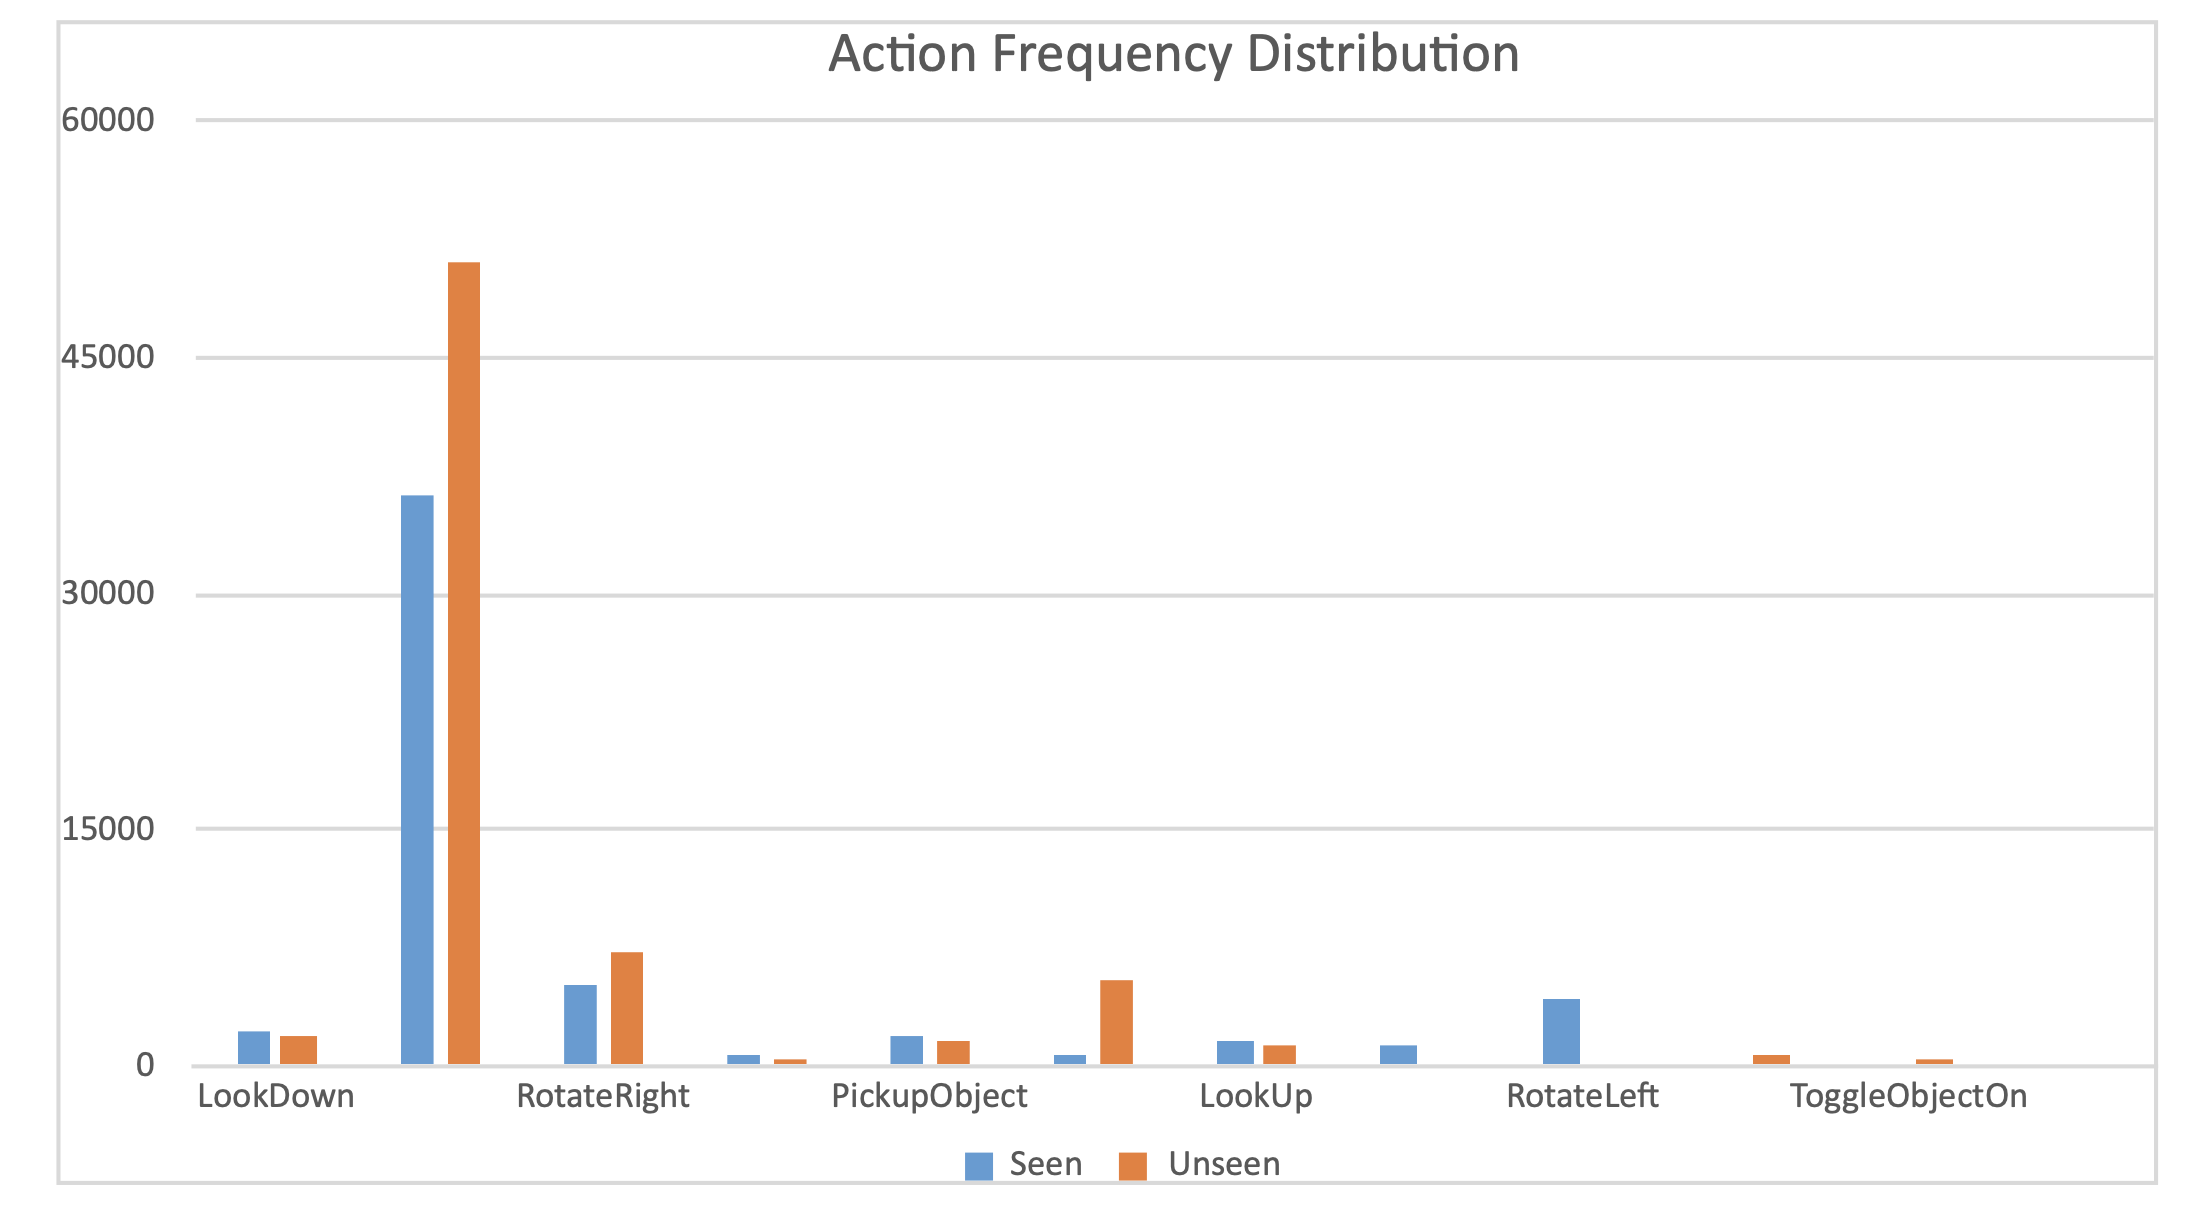
\includegraphics[width=\linewidth]{Reports/4-Analysis-of-Baselines/ac_freq.png}
    \caption{Action frequency distribution. Some bars on the x-axis are missing their label. The following are the labels from left to right: LookDown, MoveAhead, RotateRight, OpenObject, PickupObject, CloseObject, LookUp, PutObject, RotateLeft, SliceObject, ToggleOn, ToggleOff }
    \label{fig:act_freq}
\end{figure*}

\paragraph{Action Dependencies}

 For the MOCA model, we analyze the effect that the previous action prediction has on the distribution of the next prediction in figure \ref{fig:MOCA_codep}. To allow for comparison we also display the action-action dependencies for the human-labelled sequences in figure  \ref{fig:GROUND_codep} and for the ALFRED baseline model in \ref{fig:ALFRED_codep} . In every heatmap, the previous action is shown on the left axis and the predicted action is shown on the vertical axis. Interestingly, the heatmaps show the fact that both the MOCA and ALFRED baseline models struggle to correctly predict the ``CloseObject'' action after the ``PickupObject'' action. 
 
  \begin{figure*}
    \centering
    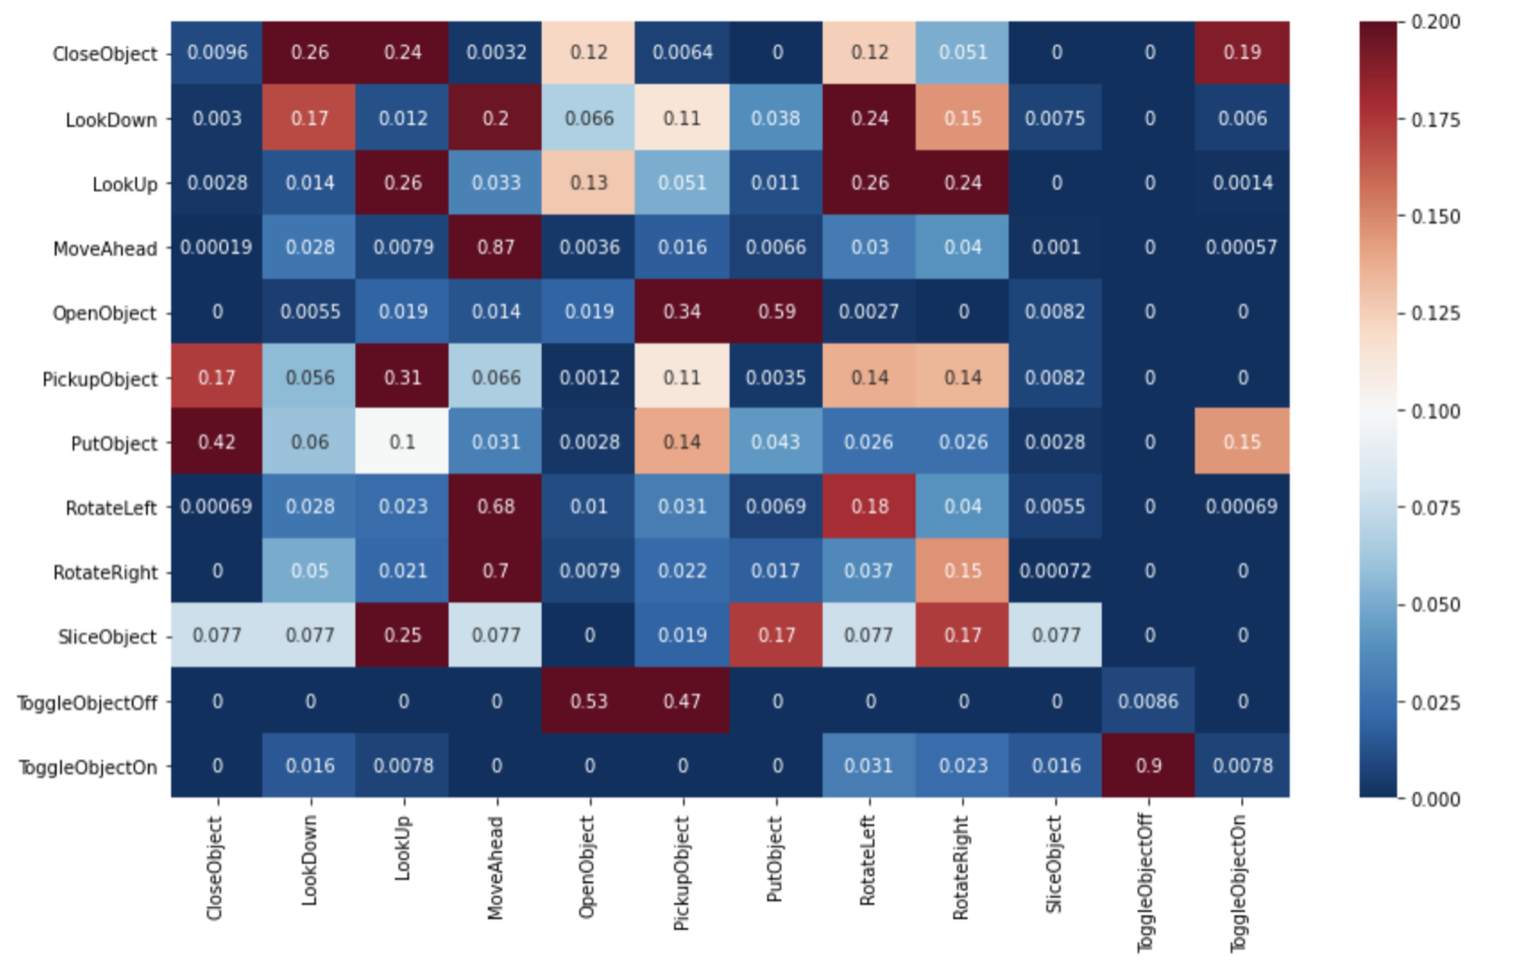
\includegraphics[width=\linewidth]{Reports/4-Analysis-of-Baselines/ALFRED_codep.png}
    \caption{Action dependency heatmap for the ALFRED baseline}
    \label{fig:ALFRED_codep}
\end{figure*}
 
 \begin{figure*}
    \centering
    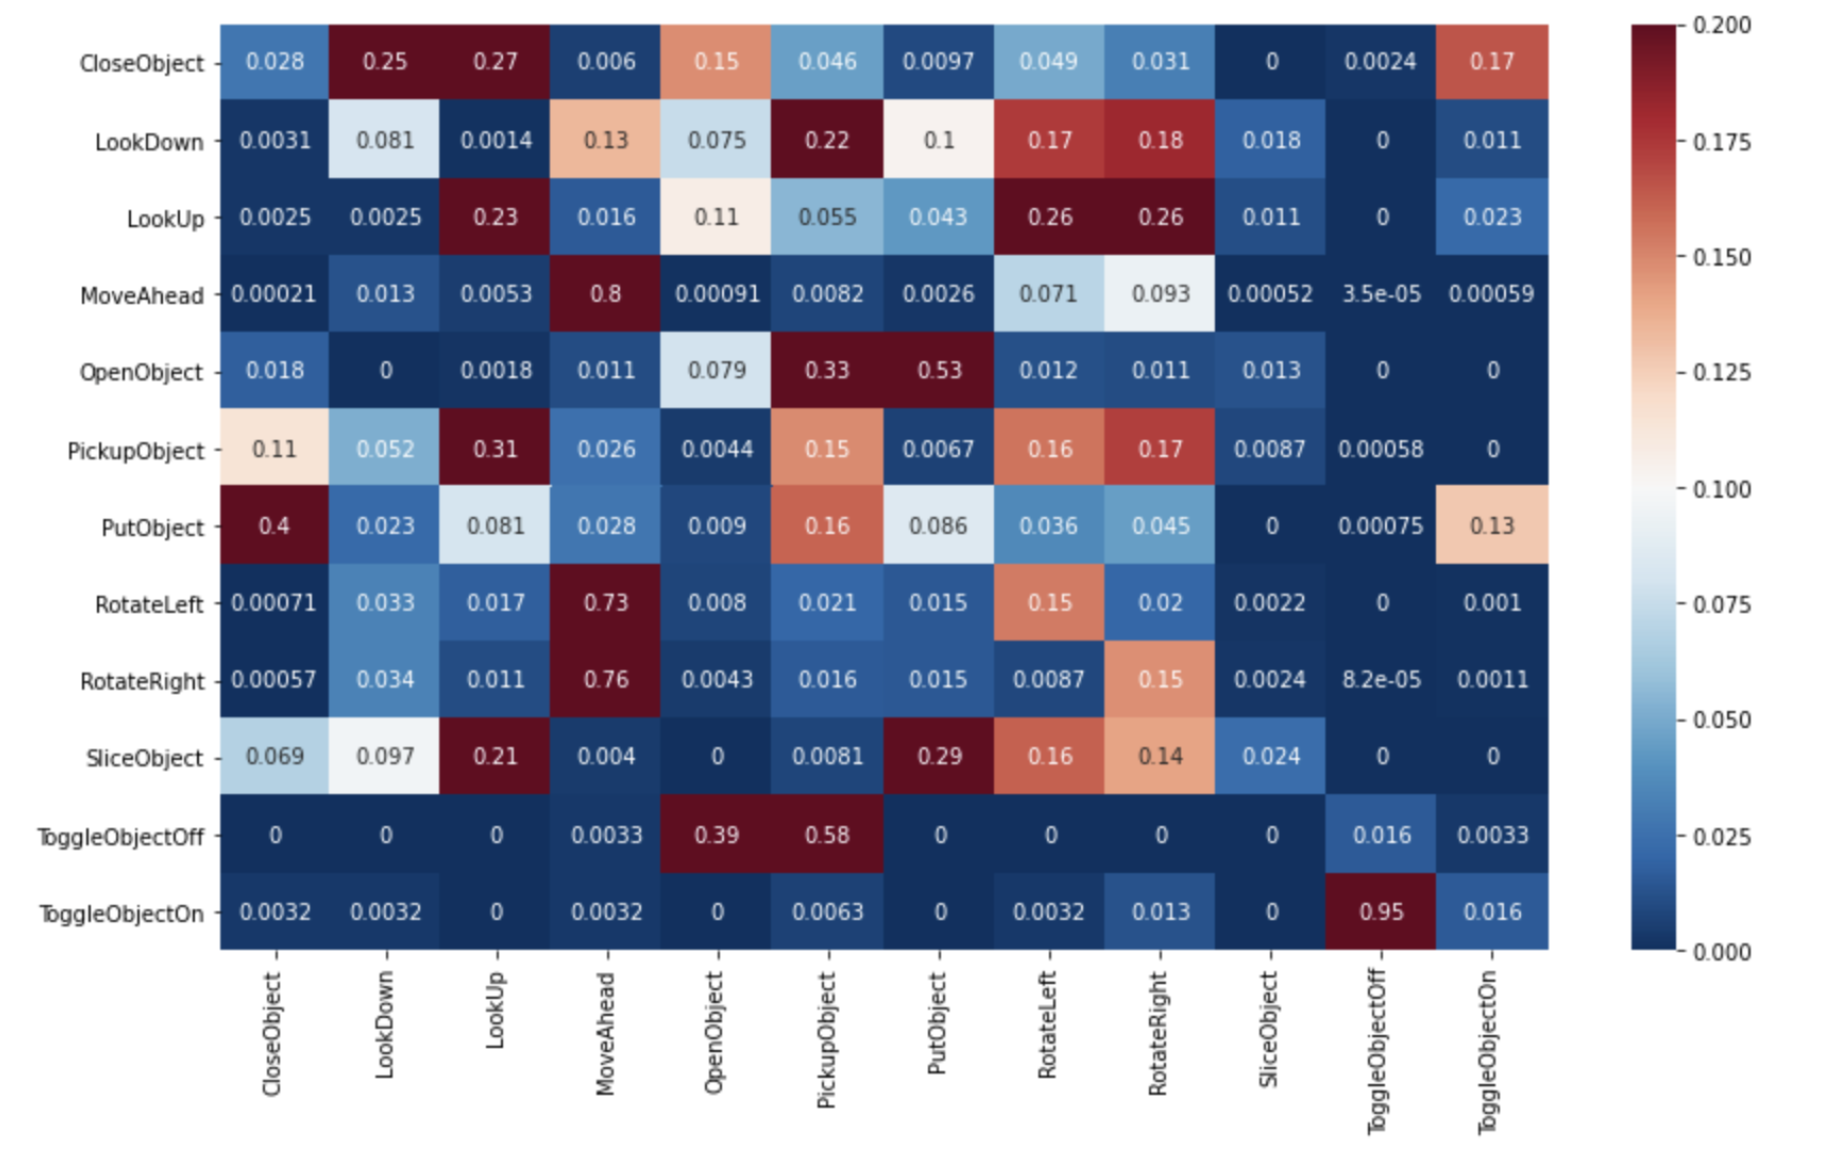
\includegraphics[width=\linewidth]{Reports/4-Analysis-of-Baselines/MOCA_codep.png}
    \caption{Action dependency heatmap for the MOCA model}
    \label{fig:MOCA_codep}
\end{figure*}

 \begin{figure*}
    \centering
    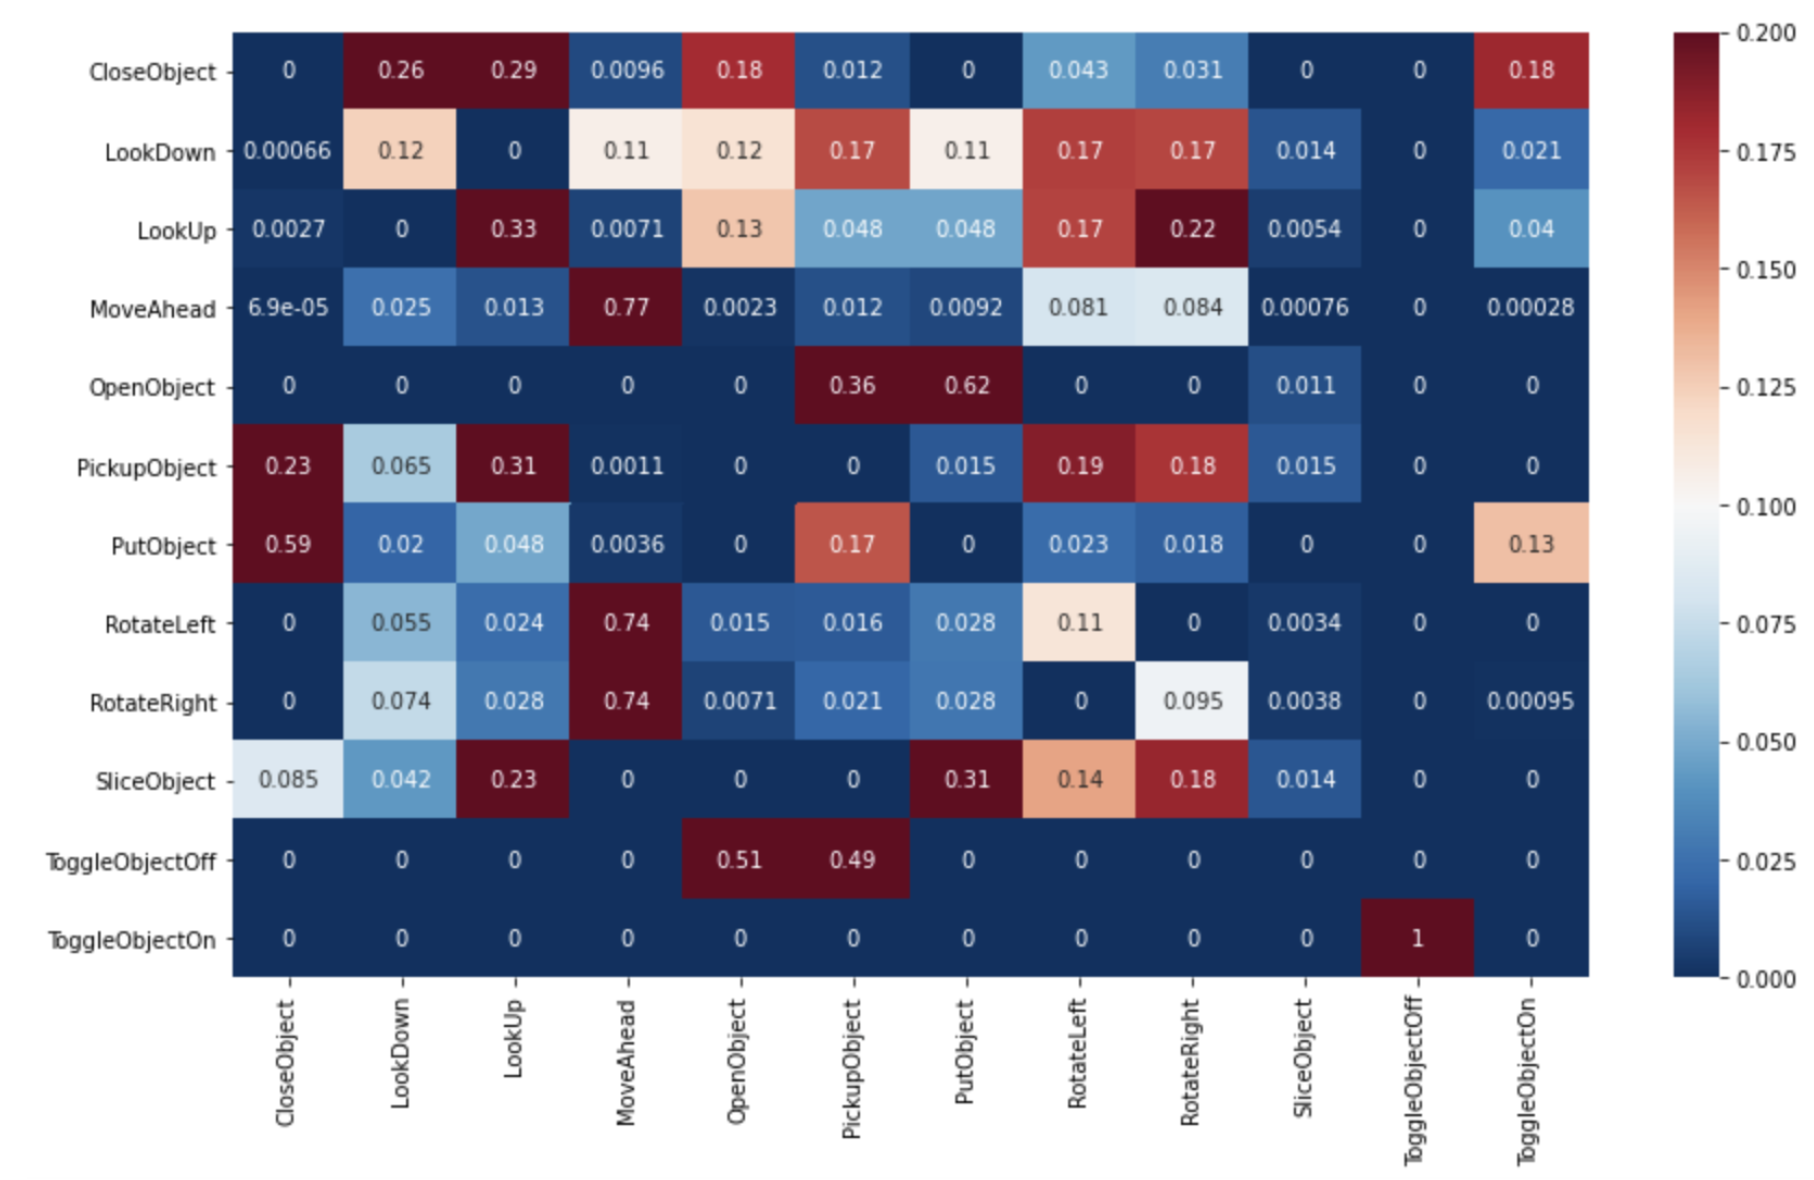
\includegraphics[width=\linewidth]{Reports/4-Analysis-of-Baselines/GROUND_codep.png}
    \caption{Action dependency heatmap for human-labelled sequences}
    \label{fig:GROUND_codep}
\end{figure*}



\section{Segmentation}

Interaction tasks (non-navigational) use an output segmentation mask to specify the object to interact with. In this section, we analyze the performance of these mask predictions. Intersection over union (IoU) is a metric for the overlap between two regions. We calculate the IoU between the output masks predicted by the MOCA model and the ground truth masks. We also explore how the proportion of output segmentation masks with IoUs  changes at various threshold of IoU. The results are displayed in table \ref{tab:seg_acc}. In general, the IoU is significantly larger for seen task environments than for unseen task environments. This highlights the problem of generalization of the vision component of the model.

In addition to the IoU we observe in our error analysis table for the MOCA model (Table \ref{tab:error_analysis}) that a large portion of invalid actions (about 40\%) are due to the object being visible but incorrectly located in the image by the interaction mask. This indicates that improving the component of the model that generates the interaction masks could lead to significant improvements in the overall performance of the model.



\begin{table}[]
\centering
\begin{tabular}{lll}
        & Unseen & Seen  \\
Avg IoU & 0.474  & 0.602 \\
Acc@0.0 & 0.467  & 0.684 \\
Acc@0.1 & 0.396  & 0.651 \\
Acc@0.2 & 0.355  & 0.616 \\
Acc@0.3 & 0.318  & 0.582 \\
Acc@0.4 & 0.288  & 0.541 \\
Acc@0.5 & 0.247  & 0.486
\end{tabular}
\caption{Average IoU and accuracy at 6 different IoU thresholds for the MOCA model.}
\label{tab:seg_acc}
\end{table}



\section{Error Analysis}
In the Alfred world, actions are not always valid. This might be due to a variety of reasons, for example, objects could be blocking the movement of the agent, or an object the agent wants to interact with might not be present in the image.   
In Table \ref{tab:error_analysis}, we report statistics on the reason why certain actions are considered invalid for the MOCA model. Our first observation is that in the seen scenes  the vast majority (80\%) of invalid actions are from two categories: the agent is unable to move (blocked) and the object was visible but not located correctly. In the unseen scenes this trend in the errors is even more accentuated with   87\% of the errors being from these two categories  (47\% for the agent being blocked, and 40\% for the object not being located correctly). These results indicate possible areas for improvement.

Furthermore, in the second part of the Table \ref{tab:error_analysis}, we observe that 28\% and 40\% of trajectories are interrupted because they reach the limit of 10 errors (for seen and unseen scenes respectively). This indicates that the presence of many invalid actions causes a large portion of failures. The two major areas for improvement in this direction are: 1. spatial detection of the validity of an action and 2. visual detection of objects.

We also manually observed such examples, and it appeared that in a significant portion of these examples the agent appeared to be stuck in between objects with repeated movement obstructions. This indicates that the agent is frequently unable to get unstuck. 

\begin{table*}[]
\centering

\begin{tabular}{|l|c|c|c|c|}
\hline
                                             & \multicolumn{2}{c|}{Seen} & \multicolumn{2}{c|}{Unseen} \\ \hline
                                             & Failure     & Success     & Failure      & Success      \\ \hline
Agent blocked                                & 1514        & 139         & 2639         & 7            \\ \hline
Agent state not allowed                      & 127         & 2           & 79           & 0            \\ \hline
Object visible but not located correctly     & 1569        & 28          & 2191         & 3            \\ \hline
Object not found in scene                    & 96          & 0           & 202          & 4            \\ \hline
Object property not allowed                  & 170         & 9           & 102          & 2            \\ \hline
Others                                       & 163         & 0           & 124          & 0            \\ \hline
Target state not allowed                     & 105         & 0           & 46           & 0            \\ \hline
No valid target                              & 40          & 0           & 25           & 0            \\ \hline
Object not visible                           & 109         & 3           & 153          & 0            \\ \hline
Object state not allowed                     & 21          & 0           & 18           & 2            \\ \hline
                                             &             &             &              &              \\ \hline
Frequency of error limit (10 errors) reached & 0.28        &             & 0.40         &              \\ \hline
Number of Errors (when less then 10 errors)  & 4.44        &             & 4.91         &              \\ \hline
Average number of errors                     & 6.03        & 1.05        & 6.99         & 0.78         \\ \hline
Average length of sequences of errors        & 2.954       & 1.19        & 3.57         & 1.17         \\ \hline
\end{tabular}
\caption{Analysis of types of error messages returned by Thor for invalid actions. We compare failed and successful tasks as well as unseen and seen scenes. The first part of the table contains counts of errors of different types across the validation dataset. The second part computes statistics about the number of errors per trajectory.}
\label{tab:error_analysis}
\end{table*}


\section{Unimodal Analysis}

Both the MOCA and ALFRED baselines are tested in 4 identical ablation studies which restrict the input to the model. We report the results of the ablation studies performed by authors in Table \ref{tab:results}. ``No Visual'' refers to not having access to any visual input.  The ``No Language'' setting removes all textual input to the model so that the model has to guess the task based on the visual input. ``Goal only'' refers to only having access to the visual input and the overall task objective without the step-by-step  instructions. ``Instruction Only'' refers to having access to the visual input and the low-level step-by-step instruction without the overall task objective. We observe that for the ALFRED Seq2Seq baseline in the seen scenes there is benefit in having access to different modalities. However, in the unseen scenes, the performance on the single modalities is equal (in one case even greater) than the performance using all modalities. This indicates that

In the MOCA baseline we observe that especially in the unseen scenes all modalities are important to obtain high performance. This indicates that there is a certain degree of cross-modality reasoning that the model is able to perform.
One of the key insights from the ablation studies is that the MOCA paper makes far superior predictions when textual input is limited (No language and goal-only). An explanation is that the MOCA model is able to memorize the relationship between objects and the actions that are frequently performed upon them.




\section{Discussion and Conclusion}
In this report we provide the results of the analysis of two baseline models for the ALFRED task, with a particular emphasis on MOCA. We believe that the following conclusion from our analysis could inform future work to improve the MOCA model:
\begin{enumerate}
    \item Unseen scene generalization is an issue. The performance of the models drops significantly between seen and unseen scenes highlighting the problem of generalizing to new environments.
    \item Trajectories reaching the invalid action limit of 10 correspond to a large portion of errors (30\% for seen, 40\% for unseen tasks). 
    \item The two major reasons for invalid actions are the agent being blocked, and the object being incorrectly located in the image even though it is visible.
    \item The agent fails to have a good model of the validity of movements, especially in unseen scenes. This might be due to a mismatch in the training and testing environments. We hypothesize that during training the agent might have seen few cases of being stuck or having an obstruction.
    \item The agent could improve its ability to recognize objects in an image. 
\end{enumerate}




\clearpage
% Please use 
\bibliographystyle{acl_natbib}
\bibliography{references}

%\appendix



\end{document}
